\chapter{Indledning} \label{cph:indledning}

\noindent Når man bor i et bofællesskab, kommer der ofte mange bolde, som skal holdes i luften. Der er et fælles ansvar for bofællesskabet, som indebærer flere ting: Hvem skal rengøre huset, og hvornår skal det gøres? Hvem har vaskemaskinen kl 16? Er der en fælles madplan, og hvem er med i den? Kommer familien på besøg, eller er der fest i weekenden og mange andre ting der internt skal koordineres. For at hjælpe med at holde disse bolde i luften, udvikles WePlanner, som har til formål at optimere håndteringen af ovenstående problematikker i et bofællesskab.

%Det er svært at koordinere med hinanden verbalt, da folk har travlt med deres hverdag, hurtigt glemmer beskeder og måske ikke ender med at få en besked ud til alle personer. På baggrund af dette har projektet til formål at optimere håndteringen af de ovenstående temaer.

%\noindent I dette projekt er der derfor blevet gjort fokus på at lave en webapplikation til bofællesskaber, som vil være et centralt sted til at kommunikere, planlægge og strukturere dagligdagen for bofællesskabet. Dette projekt bliver kaldt for WePlanner.

\section{Problemformulering}\label{sec:problemformulering}
Med udgangpunkt i projektets formål er der i gruppen kommet frem til følgende problemformulering:
\begin{center}

\textit{"Hvordan kan man med en webapplikation hjælpe med planlægningsmæssige}\\
\textit{problematikker i bofællesskaber og evt. andre sociale sammenhænge?"}
% \vspace{5mm}\\\textbf{Not so good:}

\end{center}

\noindent Med udgangspunkt i problemformulering, er det ønsket fra projektgruppens side at udvikle produktet \textit{WePlanner}.

\section{Produktbeskrivelse}
\noindent WePlanner er en webapplikation som gør det nemmere for fællesskaber, at kunne kommunikere med hinanden. I den første udgave af webapplikationen, er der lagt fokus på at lave et fuldendt planlægningsværktøj for bofællesskaber og kollegier, og senere hen udvikle det til at kunne bruges i andre sociale sammenhænge.

En bruger opretter sig på hjemmesiden, og kan nu oprette en gruppe for sit fællesskab, eller blive inviteret via. E-mail, til en allerede eksisterende gruppe. Den bruger der opretter gruppen, er automatisk ejer af gruppen, og har dermed flere rettigheder end de andre brugere. Flere brugere kan godt blive gjort til administrator af gruppen.

Når gruppen er oprettet, kan brugere tilføje widgets til denne gruppe, som hver især har forskellige egenskaber. Når man er inde på gruppens forside, vises alle de tilføjede widgets med en overskrift, og den vigtigste information fra den enkelte widget. På denne måde kan man udefra gruppens forside, få et godt overblik af relevant information. Ved at klikke på en widget, udvides denne og al information kan findes heri.

\noindent De widgets der i første omgang skal udarbejdes er følgende:

\begin{itemize}
\item  \textbf{Kalender}

Her kan brugere tilføje begivenheder, som er relevant for de andre brugere i gruppen. Kalenderen kan bruges til at få et overblik over begivenheder for et fællesskab, eller en bruger.
\end{itemize}

\begin{itemize}
\item  \textbf{Pinned event}

Bruges til at fremhæve en begivenhed, hvis den er meget vigtig.
\end{itemize}


\begin{itemize}
\item  \textbf{Booking}

Her kan brugere gå ind og reservere ressourcer og se, hvornår en ressource er reserveret. Dette kan f.eks. bruges til at lave et bookingsystem af en fælles vaskemaskine.
\end{itemize}

\begin{itemize}
\item  \textbf{Planlægning}

Denne bruges til at lave planlægning over faste opgaver. Brugere kan gå ind og se, hvornår det er deres tur, og bytte deres vagter med de andre brugere. Dette kan f.eks. bruges til at lave en mad- eller rengøringsplan.
\end{itemize}

\begin{itemize}
\item  \textbf{Liste}

\noindent Kan bruges til at oprette en liste, som brugerne kan tilføje elementer til. Denne kan f.eks. bruges til at lave en fælles indkøbsliste.
\end{itemize}

\begin{itemize}
\item  \textbf{Betaling}

\noindent Her kan en bruger skrive ind, hvis han/hun har lagt ud for noget, som nogle af de andre brugere skal betale for. De betalende brugere går ind og markerer, når de har betalt, og den betalende bruger accepterer, at der er betalt tilbage.
\end{itemize}

\begin{itemize}
\item  \textbf{Opslagstavle}

\noindent Her kan brugere skrive et opslag, som kan være relevant for de andre brugere. Denne widget kan som den eneste deles med andre grupper. På den måde kan den fungere som en fælles opslagstavle for en hel opgang, uden at opgangen skal have en fælles gruppe.
\end{itemize}

\noindent Widgets som tilføjes, har hver deres indstillingsmuligheder, så de kan tilpasses efter gruppens behov. 

\subsection{Visualisering af produkt}
For at tydeliggøre, hvordan idéen visuelt ser ud, er der herunder lavet nogle udkast til at understøtte dette. Herunder på figur \ref{fig:login_site} er login-siden vist. Det er det første man, som bruger møder. Det er her muligt at logge ind med sin e-mail og password. Derudover er det også muligt at oprette en bruger, selvom dette ikke er vist.
\begin{figure}[H]
  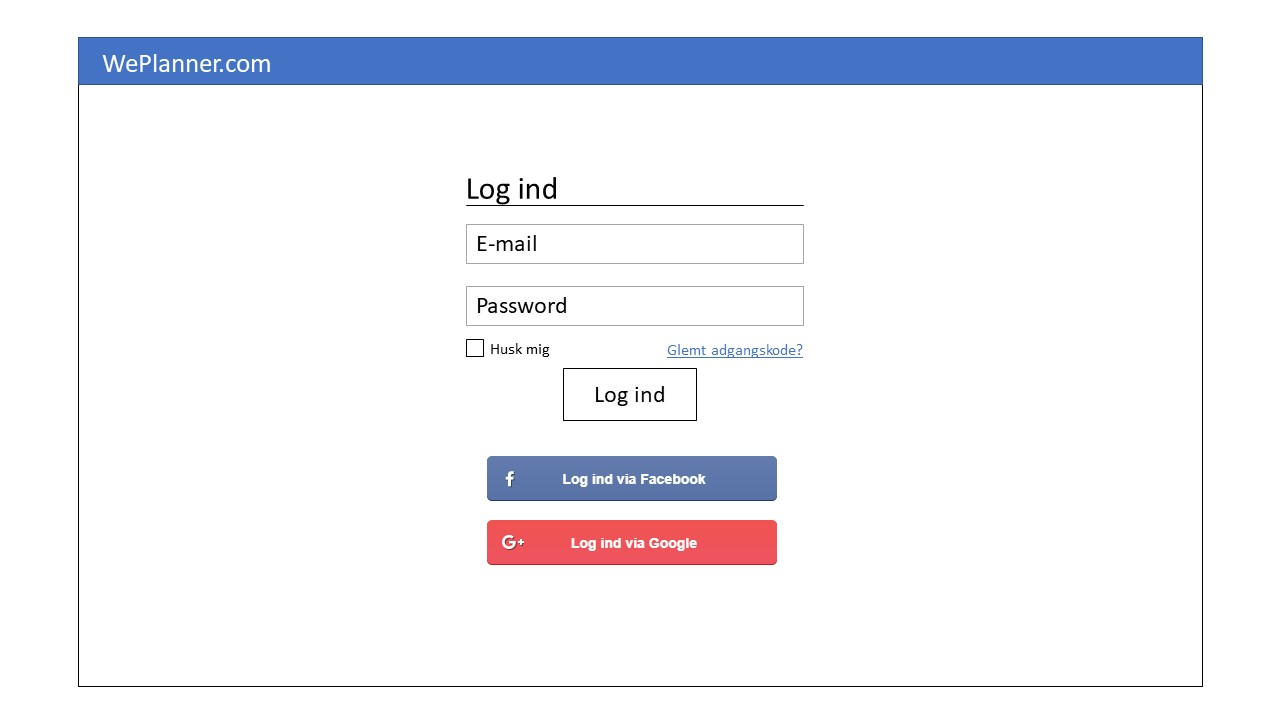
\includegraphics[width=\linewidth]{01_Billeder/04_Indledning/Slide1.JPG}
  \centering
  \caption{Login side}
  \label{fig:login_site}
\end{figure}

\noindent Når man er logget ind med sin bruger, møder man 'Home' siden, som kan ses på figur \ref{fig:home_site}. Her kan brugeren se alle de grupper, hvor brugeren er medlem. Derudover har brugeren også mulighed for at oprette en gruppe.
\begin{figure}[H]
  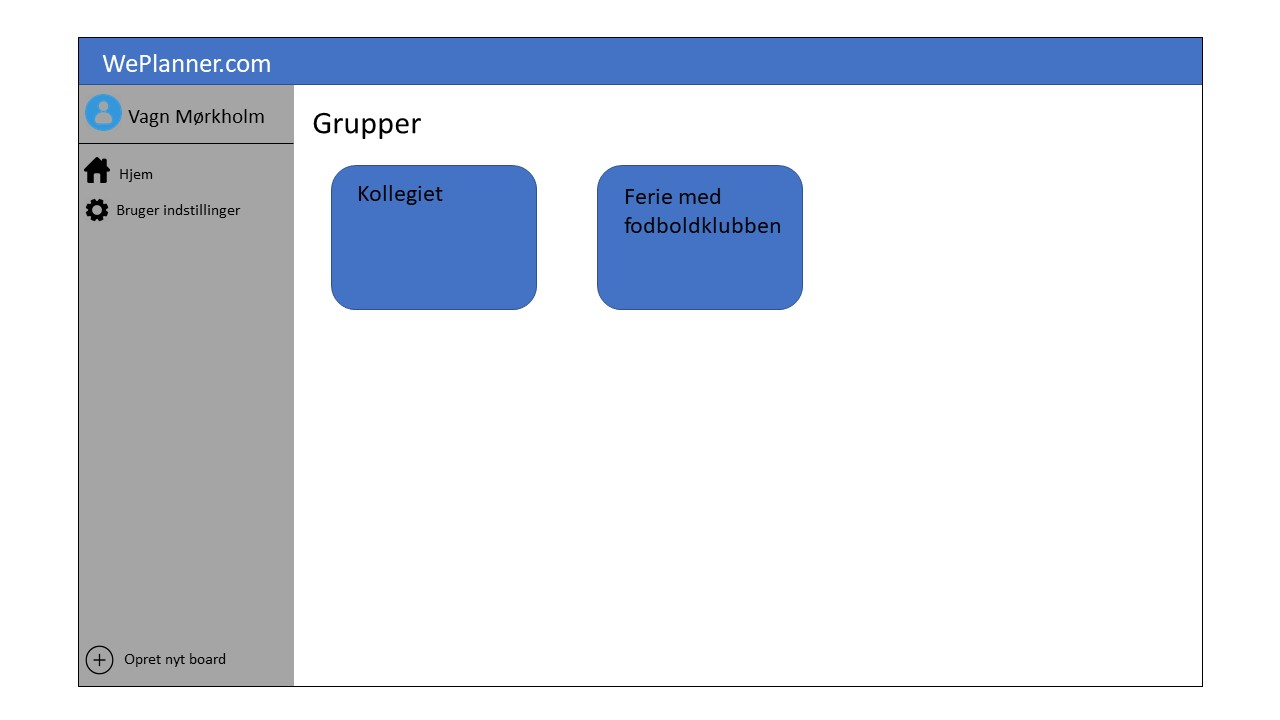
\includegraphics[width=\linewidth]{01_Billeder/04_Indledning/Slide2.JPG}
  \centering
  \caption{Home side}
  \label{fig:home_site}
\end{figure}

\noindent Ved at vælge en gruppe, kommer man ind på en ny side, som viser gruppens widgets. Her kan brugeren få et hurtigt overblik ved at kigge på de forskellige widgets. Brugeren kan så trykke på en widget, for at få vist flere informationer. Dette ses på figur \ref{fig:board_site}.
\begin{figure}[H]
  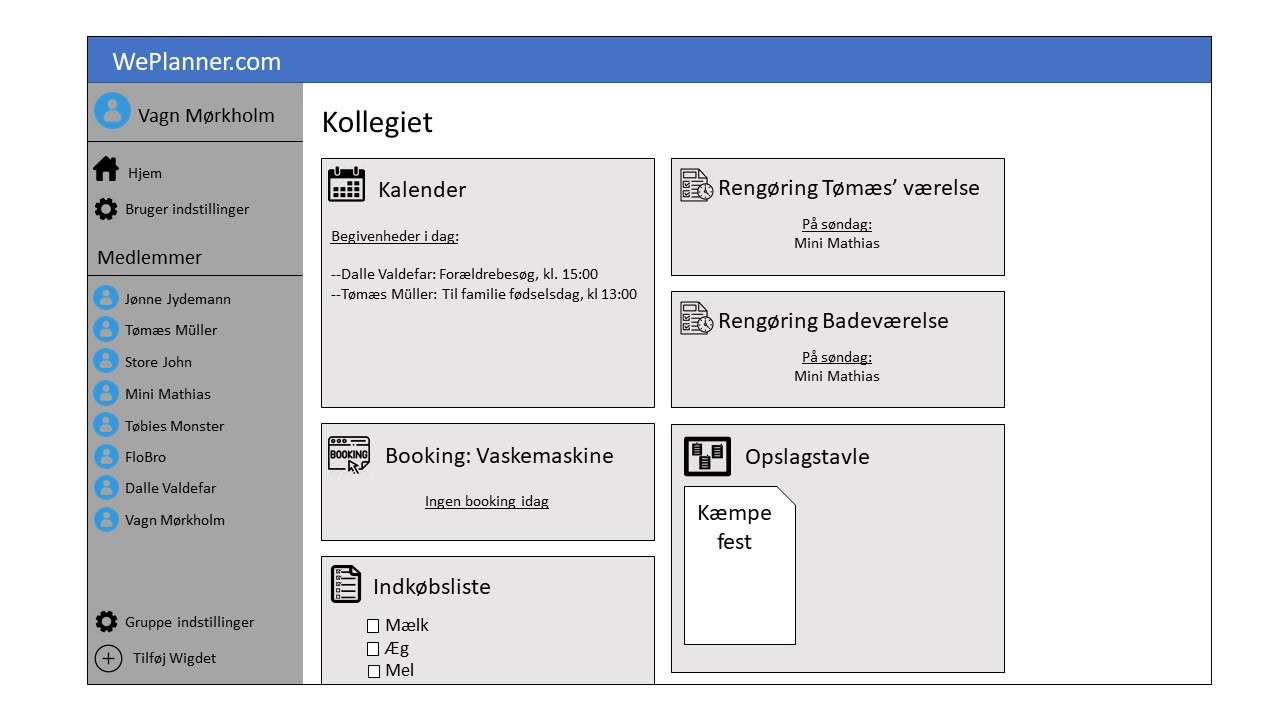
\includegraphics[width=\linewidth]{01_Billeder/04_Indledning/Slide3.JPG}
  \centering
  \caption{Gruppeside}
  \label{fig:board_site}
\end{figure}


\section{Prototype}
Der er købt et domæne der har navnet: www.weplanner.dk. I bilag findes en brugervejledning til, hvordan der kan navigeres rundt i web-applikationen. \valdemar{Reference til bilag} Brugervejledningen indeholder også et demo-login for en bruger, der er med i nogle grupper. Dette skulle gerne give et eksempel på, hvordan det var tænkt at weplanner kunne anvendes i virkeligheden. 

\section{Afgrænsninger}
For at begrænse projektets indhold til en passende størrelse, foretages en afgrænsning af projektet. Dette gør det muligt at fastlægge nogle krav, som der kan tages udgangspunkt i udviklingsprocessen. Disse kan da prioriteres ud fra forskellige parametre som tid, forhåndskendskab og vigtighed, hvorved udviklingsprocessen kan struktureres efter denne prioritering. For at lave denne afgrænsning, foretages en MoSCoW analyse, som kan ses i afsnit \ref{sec:MoSCoW}.

\subsection{MoSCoW} \label{sec:MoSCoW}
I starten af udviklingsforløbet foretages en MoSCoW analyse, for at få et overblik over applikationens ønskede funktionalitet, samt for at prioritere implementeringen af applikationens elementer. Resultatet af denne analyse kan ses herunder.

\noindent \textbf{Must have:}
\begin{itemize}
    \item Applikationen skal have en login-funktion og mulighed for at oprette brugere
    \item En bruger skal identificeres ved e-mail som anvendes ved login
    \item I applikationen skal det være muligt at oprette en gruppe med et default layout, hvortil der kan tilføjes medlemmer
    \item Administrator rettigheder for grupper
    \item Applikationen skal indeholde en kalender
    \item Applikationen skal indeholde funktionalitet der gør det muligt at se og planlægge en madplan og rengøringsplan.
    \item Det skal være muligt at bytte vagter mellem brugere. 
    \item Gruppens aktiviteter skal vises på gruppens kalender.
    \item Applikationen skal indeholde en opslagstavle for en gruppe.
    \item Der skal kunne oprettes forbindelse til serveren ved brug af HTTP.
    \item Applikationen skal indeholde en liste widget.
    \item Det skal være muligt for gruppens medlemmer at tilføje widgets på gruppens side.
    \item Det skal være muligt for en gruppes administrator at fjerne/redigere i widgets på gruppens side.
    \item Applikationen skal gøre det muligt at oprette et booking system til reservation af ressourcer.
    \item Applikationen skal have en regnskabs widget.
\end{itemize}

\noindent \textbf{Should have:}
\begin{itemize}
    \item Brugere skal kunne modtage notifikationer om ændringer i widgets.
    \item Mulighed for at tilpasse udseendet af gruppen.
    \item Owner rettigheder for grupper.
    \item Projektets applikation hostes på dens eget domæne.
\end{itemize}

\noindent \textbf{Could have:}
\begin{itemize}
    \item Mulighed for at indsamle brugerstatistikker.
    \item Flere loginmuligheder via social media-accounts.
    \item Mulighed for at vælge andre sprog.
\end{itemize}

\noindent \textbf{Won't have (this time)}
\begin{itemize}
    \item En tilsvarende App til iOS/Android.
    \item Integrering med mobilePay/ weshare mm.
    \item Integrering med dansk supermarked der udbyder levering af varer.
    \item Søgemaskine optimering.
\end{itemize}



\section{Udviklingsværktøjer}

\subsection{Microsoft Visual Studio}
WePlanner gør brug af Microsoft Visual Studios \valdemar{reference} indbyggede MVC arkitektur for ASP.NET. Dette betyder at WePlanners filstrukturer er struktureret efter Models, Views og Controllers.

\subsection{ASP.NET Core}
WePlanners backend er implementeret i ASP.NET Core 2.2, som er platformsuafhængig. \valdemar{reference} 

\subsubsection{Identity Framework}
Identity Framework \valdemar{indsæt reference} tilføjes til projektet, der tilføjer funktionalitet der bla. gør det muligt at registrere brugere og logge ind, uden at dette skal implementeres selv.

\subsection{Entity Framework Core}
Entity Framework Core anvendes, da gruppen har erfaring med det fra faget I4DAB \cite{DAB}, samt fordi det ligesom ASP.NET Core, er platformsuafhængigt.
